\documentclass[11pt]{article}
\usepackage[utf8]{inputenc}
\usepackage{amsmath}
\usepackage{amssymb}
\usepackage{fancyhdr}
\usepackage{systeme}
\usepackage{geometry}
\usepackage{multicol} %for multiple columns
\usepackage{graphicx,color} % Graphics, Figures
\usepackage{xcolor} %color
\usepackage{tikz}
\usepackage{pgfplots}
\usepackage{caption}
\usepackage{subcaption}
\usepackage{float}
\usetikzlibrary{shapes,positioning,intersections,quotes}
\pgfplotsset{compat=1.16}
\usepackage[most]{tcolorbox}
\usepackage{multicol}
\usepackage{multirow}

\geometry{left=20mm, right=20mm, top=30mm, bottom=25mm}
\pagestyle{fancy}
\lhead{Quadratic Equation}
\rhead{By P'Jashan}
\tcbset{colback=yellow!10!white, colframe=red!50!black, 
        highlight math style= {enhanced, %<-- needed for the ’remember’ options
            colframe=red,colback=red!10!white,boxsep=0pt}
        }


\begin{document}
\begin{center}
    \textbf{\huge Quadratic Equation}
\end{center}
A \emph{quadratic equation} is an equation in the form  $ax^2+bx+c=0$ where $a\neq 0,b,$ and $c$ are constants. For example,  $4x^2-2x+3=0$ or $3x^2=5-x$

This equation has a closed-form solution. Meaning, you can always solve the quadratic equation using formula. However, we must know other ways to solve in order to understand the formula. 
\section{Methods for solving quadratic equations}
\begin{enumerate}
    \item Factorise into linear factors.
    \begin{itemize}
        \item equation in the form  $ax^2+bx=0$
        This is the easiest form to solve, we can see that $x$ is a common factor. 
        \begin{gather*}
            ax^2+bx=0
            \\x(ax+b)=0
            \\x=0 \hspace{2mm} \text{or} \hspace{2mm} ax+b=0
        \end{gather*}
        Therefore, the solutions are $x=0,-\frac{b}{a}$
        \vspace{5mm}
        \item equation in the form $x^2+bx+c=0$ (Note that it's the general form when $a=1$).
        Suppose $x^2+bx+c$ can be factorized as
        \begin{align*}
            x^2+bx+c=(x+p)(x+q)
            \\ = x^2+qx+px+pq
            \\ = x^2+(p+q)x+pq
        \end{align*}
        Then, by comparing LHS and RHS, we have $p+q=b$, $pq=c$. Therfore, solving equation in this form, we \textcolor{blue}{find $p,q$ such that $p+q=b$ and $pq=c$} 
        \vspace{5mm}
        \item equation in the form $ax^2+bx+c=0$ where $a\neq 1$ \\
        The steps are as follows
        \begin{itemize}
        \renewcommand\labelitemii{$\rightarrow$}
            \item find $p,q$ such that $pq = a$
            \item find $r,s$ such that $rs = c$
            \item $b = qr+ps$
            
                \begin{center}
                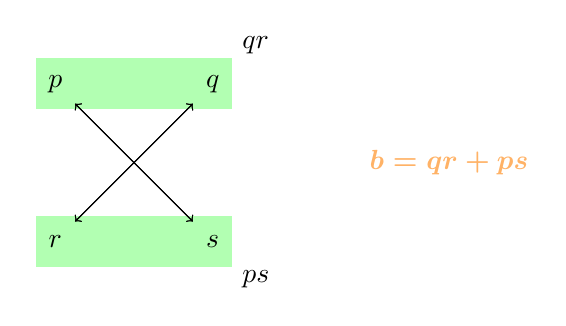
\begin{tikzpicture}[
                roundnode/.style={circle, draw=blue!60, fill=blue!5, very thick, minimum size=7mm},
                squarednode/.style={rectangle, draw=red!60, fill=red!5, very thick, minimum size=5mm},
                ]
                %Nodes
                \node[rectangle,minimum width = 2.5cm,minimum height=0.65cm,fill=green!30!white]      (F) at (1,0) {};
                \node[rectangle,minimum width = 2.5cm,minimum height=0.65cm,fill=green!30!white]      (G) at (1,-2) {};
                \node[circle,minimum size = 7mm]        (H) at (0,0) {$p$};
                \node[circle,minimum size = 7mm,label=above right:{$qr$}]        (I) at (2,0) {$q$}; 
                \node[circle,minimum size = 7mm]        (J) at (0,-2) {$r$}; 
                \node[circle,minimum size = 7mm,label=below right:{$ps$}]        (K) at (2,-2) {$s$}; 
                \node[rectangle]        (L) at (5,-1) {\textcolor{orange!60!white}{$\boldsymbol{b=qr+ps}$}};

                %Lines
                \draw[<->] (H) -- (K);
                \draw[<->] (I) -- (J);
                \draw[<->] (H) -- (K);
                \draw[<->] (I) -- (J);
                \end{tikzpicture}
                \end{center}
            \item Then the equation can be factorised as $ax^2+bx+c=(px+q)(rx+s)$
        \end{itemize}
    \end{itemize}
    \textcolor{red}{*This method is very easy if $p,q,r,s \in \mathbb{Z}$}
    \newpage
    \item Solve by completing the square.\\
    This method allow us to solve any quadratic equations. We first recall that $(a+b)^2=a^2+2ab+b^2$ then,consider the equation in the form $x^2+bx+c=0$. Our objective is to rearrange the equation to the form $(x+h)^2=k$. That is 
    \begin{gather*}
        x^2+bx=-c 
        \\ x^2+2(x)\left(\frac{b}{2}\right)+\left(\frac{b}{2}\right)^2 = -c+\left(\frac{b}{2}\right)^2
    \end{gather*}
    \begin{equation}
        \label{eqn:eqn1}
        \left(x+\frac{b}{2}\right)^2=\left(\frac{b}{2}\right)^2-c
    \end{equation}
    equation (\ref{eqn:eqn1}) is solvable if and only if $\text{RHS}=\left(\frac{b}{2}\right)^2-c \geq 0$ ($\because$ squares of any real number is non-negative)
    
    \item Quadratic formula.\\
    Sometimes, solving quadratic equations by factorisation or completing the square can be long and difficult. In that case, we may use the quadratic formula:
    \begin{equation*}
        \text{If} \hspace{2mm} ax^2+bx+c=0,
    \end{equation*}
    \begin{equation*}
        \text{then} \hspace{2mm} \tcboxmath{x=\frac{-b \pm \sqrt{b^2-4ac}}{2a}}
    \end{equation*}
\end{enumerate} 

\section{Discriminant of a quadratic}
We define $\Delta = b^2-4ac$ as the 'discriminant' which is the quantity under the square root sign in the quadratic formula. The name was given because $\Delta$ can discriminate different scenarios, in this case, it gives information about \emph{number of real solutions} of the quadratic equation.
\begin{itemize}
    \item if $\Delta >0$, then there are \textbf{two distinct real roots}
    \begin{equation*}
        x=\frac{-b + \sqrt{\Delta}}{2a} \hspace{1mm}, \hspace{1mm} \frac{-b - \sqrt{\Delta}}{2a}
    \end{equation*}
    \item if $\Delta=0$, then $x=-$\scalebox{1.3}{$\frac{b}{2a}$} is the \textbf{only solution} (a \textbf{repeated} or \textbf{double root})
    \item if $\Delta<0$, then there are \textbf{no real roots}
\end{itemize}
\newpage
\section{Sign diagram}
A sign diagram is a diagram representing signs of some quantity with different values of variable.
\vspace{3mm} \\ Example 1: Draw a sign diagram of $k+6$
\vspace{1mm}\\ \underline{Solution} \hspace{2.5mm} First, find the point where $k+6=0 \hspace{1mm} \Rightarrow \hspace{1mm} k=-6$

\hspace{11.5mm} Next, when $k>-6 \hspace{1mm} \Rightarrow \hspace{1mm} k+6>0$

\hspace{21.5mm} when $k<-6 \hspace{1mm} \Rightarrow \hspace{1mm} k+6<0$

\hspace{11.5mm} Therefore, the sign diagram of $k+6$ is shown below.
\begin{center}
    \begin{tikzpicture}
    \begin{axis}[xlabel={$k$},
    height = 20mm,
    xtick={0},
    xticklabels={$-6$},
    xmin=-3,xmax=3,ymin=0,ymax=1.5,
    every axis plot/.append style={very thick},
    axis y line=none,
    axis x line=middle,
    axis line style={stealth-stealth},
    width=\axisdefaultwidth,
    ]
    %\draw [white, fill] (axis cs: 1.5,0.2) circle (2pt) node [below left] {\verysmall $\left(b_{\scriptscriptstyle n-2},f(b_{\scriptscriptstyle n-2})\right)$};
    %\addplot[]{-2};
    \node[circle,white,fill,label={[orange]-90:$+$},inner sep=0.1pt] at (axis cs:1.5,2.5) {P};
    \node[circle,white,fill,label={[orange]-90:$-$},inner sep=0.1pt] at (axis cs:-1.5,2.5) {P};
    %\addplot[white,fill] coordinates {(1,0)};
    \end{axis}
    \end{tikzpicture}
\end{center}
\newline
\\ Example 2: Draw a sign diagram of $(k+1)(k-2)$
\vspace{1mm}\\ \underline{Solution} \hspace{2.5mm} First, find the point where $(k+1)(k-2)=0 \hspace{1mm} \Rightarrow \hspace{1mm} k=-1,\hspace{0.5mm} 2$

\hspace{11.5mm} Next, we can split the value of $k$ into 3 cases.

\hspace{21.5mm} when $k>2 \hspace{1mm} \Rightarrow \hspace{1mm} (k+1)(k-2)>0$

\hspace{21.5mm} when $-1<k<2 \hspace{1mm} \Rightarrow \hspace{1mm} (k+1)(k-2)<0$

\hspace{21.5mm} when $k<-1 \hspace{1mm} \Rightarrow \hspace{1mm} (k+1)(k-2)>0$

\hspace{11.5mm} Therefore, the sign diagram of $(k+1)(k-2)$ is shown below.
\begin{center}
    \begin{tikzpicture}
    \begin{axis}[xlabel={$k$},
    height = 20mm,
    xtick={-1,2},
    xticklabels={$-1$,$2$},
    xmin=-3,xmax=4,ymin=0,ymax=1.5,
    every axis plot/.append style={very thick},
    axis y line=none,
    axis x line=middle,
    axis line style={stealth-stealth},
    width=\axisdefaultwidth,
    ]
    %\draw [white, fill] (axis cs: 1.5,0.2) circle (2pt) node [below left] {\verysmall $\left(b_{\scriptscriptstyle n-2},f(b_{\scriptscriptstyle n-2})\right)$};
    %\addplot[]{-2};
    \node[circle,white,fill,label={[orange]-90:$+$},inner sep=0.1pt] at (axis cs:3,2.5) {P};
    \node[circle,white,fill,label={[orange]-90:$-$},inner sep=0.1pt] at (axis cs:0.5,2.5) {P};
    \node[circle,white,fill,label={[orange]-90:$+$},inner sep=0.1pt] at (axis cs:-2,2.5) {P};
    %\addplot[white,fill] coordinates {(1,0)};
    \end{axis}
    \end{tikzpicture}
\end{center}
\newpage
\begin{left}
    \Large \textbf{Exercise}
\end{left}
\newline
\begin{enumerate}
    \item Solve the following equations by factorisation.
    \begin{multicols}{3}
        \renewcommand{\labelenumii}{\arabic{enumii})}
        \begin{enumerate}
            \item $x^2-4x+3=0$
            \vspace{30mm}
            \item $3x^2-8x-51=0$
            \item $3x^2-5=2x^2+4x$
            \vspace{30mm}
            \item $(2x-3)(x+1)=3$
            \item $10x+8=7x^2$
            \vspace{30mm}
            \item $x^2+64=16x$
        \end{enumerate}
    \end{multicols}
    \vspace{30mm}
    \item Solve the following equations by completing the square and quadratic formula.
    \begin{multicols}{2}
        \renewcommand{\labelenumii}{\arabic{enumii})}
        \begin{enumerate}
            \item $x^2-6x+3=0$
            \vspace{50mm}
            \item $2x^2-5x-3=0$
            \item $4x^2+49=-28x$
            \vspace{50mm}
            \item $(x+1)(x-3)=7$
        \end{enumerate}
    \end{multicols}
    \newpage
    \item Which of the given quadratic equations has the following properties.
\begin{multicols}{3}
    \begin{enumerate}
    %\renewcommand\labelitemi{$\rightarrow$}
    \renewcommand{\labelenumi}{\alph{enumi})}
    \item A repeated root.
    \item Rational roots.
    \item Two distinct real roots.
    \item No real roots.
    \end{enumerate}    
\end{multicols}
%\vspace{3mm}
\begin{multicols}{2}
    \begin{enumerate}
    %\renewcommand\labelitemi{$\rightarrow$}
    \renewcommand{\labelenumii}{\arabic{enumii})}
    \item $2x^2-7x-5=0$
    \vspace{30mm}
    \item $2x^2+6=12x$
    \item $3x^2+4x+1=0$
    \vspace{30mm}
    \item $8x^2+2x-3=0$
    \end{enumerate}    
\end{multicols}
\vspace{30mm}
\item For each of the following quadratic equations, find the discriminant $\Delta$ and hence draw its sign diagram. Find all values of $k$ for which the equation has:two real roots, a repeated root and no real roots.

    \begin{enumerate}
    %\renewcommand\labelitemi{$\rightarrow$}
    \renewcommand{\labelenumii}{\arabic{enumii})}
    \item $x^2+kx+4=-2k$
    \vspace{30mm}
    \item $(k+1)x^2+kx+k=0$
    \vspace{30mm}
    \item $4x^2+(2k+8)x+(4k+1)=0$
    \end{enumerate}    

\end{enumerate}
\end{document}